\chapter{Reliable Web Applications}%
\label{cha:reliable_web_applications}

\section{What is the Web?}%
\label{sec:web}

The Internet and the Web are ubiquitous technologies of our everyday lives,
that flourished around the 80's.
Inter-connected networked appeared as early as in the 60's.
ARPANET, founded by the Advanced Research Projects Agency (ARPA) in 1969,
standardized the communication protocols named TCP/IP in 1982 for its network.
These are the protocols still in use on the Internet today.
In August 1991, Tim Berners-Lee who had been working at CERN for the previous seven years,
shared a summary of his World Wide Web project,
including the HyperText Transfer Protocol (HTTP),
the HyperText Markup Language (HTML), and the first Web browser.
Social media, communication, search, news, entertainment, mapping,
shopping, learning, virtually any activity is now digital and online.
Simply put, the Web, also called World Wide Web (WWW), consists of the sum of all resources,
available through unique identifiers (URI), that we share on the Internet,
the global network carrying them.

In this chapter, we will recap the Web main evolutions,
from static content to dynamic applications,
and explain the choices we made to build reliable annotation Web applications.

\subsection{What is a Web application?}%
\label{sub:web_application}

An application, in the context of programming (/computers),
is a piece of software presenting information to a user,
usually in an actionable manner.
This includes programs like email clients, image editors, video games,
word processors, automatic translators, and virtually any functionality
available on a regular computing device.

Web resources are commonly accessible through a Web browser.
Thus, we can define a Web application as a user-facing software,
accessed through a Web browser.
As of May 2019 according to statcounter~\cite{browser-market-share},
the most used Web browsers are Google Chrome (62.7\% of global market share),
Apple Safari (15.9\%) and Mozilla Firefox (5.1\%).

The three pillars of Web applications are HTML, CSS and JavaScript.
HTML, for ``HyperText Markup Language'' is a description language
organizing a page information as a hierarchy of tagged content.
In Listing~\ref{lst:html}, a \verb|body| tag contains three other tags,
a title \verb|h1| (h for header), a paragraph \verb|p|, an image \verb|img|
and a button not yet linked to any action.
This hierarchical organization of an HTML page is call the DOM,
for Document Object Model.
CSS, for ``Cascading Style Sheet'', complements HTML by styling
the content of associated HTML documents.
Listing~\ref{lst:css} shows how one would add a left margin of 20 pixels
on all the document body, and make the h1 title red and bold.
Finally, JavaScript is a scripting language, not affiliated in any form
to the Java programming language.
It is run inside the browser to add dynamic behavior to a Web page.
In Listing~\ref{lst:js} we show how one could count and display
the number of times a user clicked on the button in the page.

\lstinputlisting[language=HTML,caption={Example HTML code.},label={lst:html}]{assets/code/html.html}
\lstinputlisting[language=CSS,caption={Example CSS code.},label={lst:css}]{assets/code/css.css}
\lstinputlisting[language=ES6,caption={Example JavaScript code.},label={lst:js}]{assets/code/js.js}

\subsection{Rich Web Application}%
\label{sub:rich_web_application}

Traditionally, websites used to present their resources in the form of a collection
of static documents, known as Web pages, linked together with hyperlinks.
The nature of Web pages would mostly be informative, visual or textual,
with very few other interactions than navigation through the site by
clicking on the links.

Today, thanks to evolutions of Web technologies that we will detail later,
Web applications have become full-fledged applications with almost
the same capabilities as desktop ones.
They feature functionalities like 3D graphics, audio processing or interactive elements,
and are sometimes called rich web applications.
Similar concepts like \comment{``progressive web applications'' (PWA)}{Not explained actually ...},
or ``single page applications'' (SPA) are also explained in the following sections.
In the next section, we will dive into the cornerstone of Web pages dynamism, JavaScript.


\section{JavaScript, formally known as ECMAScript}%
\label{sec:javascript_formally_known_as_ecmascript}

\subsection{Genesis of JavaScript}%
\label{sub:genesis_of_javascript}

In 1995, the dominating Web browser was the Netscape Navigator.
Realizing that pages dynamism was key in the competition against Microsoft's
own Web technologies, Netscape Communications recruited Brendan Eich,
with the aim of integrating a scripting language into their browser.
A first prototype was thus developed in 10 days (May 1995).
Assumably for marketing reasons, it was officially named JavaScript
when released in Netscape Navigator 2.0 beta 3.

Two years later, in June 1997, the European Computer Manufacturers Association
(ECMA) standardized the first version of ``ECMAScript'' as ECMA-262,
JavaScript being its most well-known implementation.
The ECMAScript (ES) standard has been evolving ever since.
Today, all browsers fully implement ES5, released in 2009,
and partially implement the most recent versions, ES2015,
ES2016, ES2017 and ES2018.

\subsection{Browser performance}%
\label{sub:browser_performance}

Many browser wars for dominance of market share occurred since the 90's.
In this section, we are particularly interested
in the wide performance improvements of the JavaScript engines,
starting around 2008 when Google released its Chrome browser.
On September 2, 2008, Google announced a new Web browser called Chrome~\cite{google-chrome}.
Its main selling feature was a new JavaScript engine called V8,
greatly improving the browser performances on web applications making
heavy use of JavaScript like their email client \comment{Gmail}
{should we use sans serif font for all names like \textsf{Gmail}.}
Note that performance in a browser depends on many factors
such that network latency, DOM computation, page rendering or JavaScript processing.
In this section, we will specifically focus on JavaScript execution performances.

\subsubsection{Dynamic interpretation}%
\label{ssub:dynamic-interpretation}

JavaScript was originally an interpreted language.
For each line of code, the engine would translate it into machine code,
and immediately execute it.
This means that for a loop, the same transformation from JavaScript to machine code
is repeated over and over again.
In addition, JavaScript is a dynamic language, which is both one of its
strongest points and a huge drag on execution.
Let's take the function adding two numbers
depicted in Listing~\ref{lst:add-js} as an example.

\lstinputlisting[%
	language=JavaScript,
	caption={Adding two values.},
	label={lst:add-js}
]{assets/code/add.js}

\comment{}{If what follows is a quote, it should be made clearer in the presentation.}
\begin{displayquote}
According to the ECMAScript specification~\cite{ecmascript},
the addition operator either performs string concatenation or numeric addition.
The production ``AdditiveExpression : AdditiveExpression + MultiplicativeExpression''
is evaluated as follows:

\begin{enumerate}
    \item Let lref be the result of evaluating AdditiveExpression.
    \item Let lval be GetValue(lref).
    \item Let rref be the result of evaluating MultiplicativeExpression.
    \item Let rval be GetValue(rref).
    \item Let lprim be ToPrimitive(lval).
    \item Let rprim be ToPrimitive(rval).
    \item If Type(lprim) is String or Type(rprim) is String, then
    \begin{enumerate}
        \item     Return the String that is the result of concatenating ToString(lprim) followed by ToString(rprim)
    \end{enumerate}
    \item Return the result of applying the addition operation to ToNumber(lprim) and ToNumber(rprim). See the Note below 11.6.3.
\end{enumerate}

\textbf{NOTE 1}. No hint is provided in the calls to ToPrimitive in steps 5 and 6. All native ECMAScript objects except Date objects handle the absence of a hint as if the hint Number were given; Date objects handle the absence of a hint as if the hint String were given. Host objects may handle the absence of a hint in some other manner.

\textbf{NOTE 2}. Step 7 differs from step 3 of the comparison algorithm for the relational operators (11.8.5), by using the logical-or operation instead of the logical-and operation.
\end{displayquote}


In theory, if we know that we will only use this function
to sum two numbers, it should compile to a single instruction.
However, due to the dynamic nature of JavaScript,
as specified in the standard, the code has to check if the arguments
are strings, objects, and proceed first with conversions before
eventually reaching the instruction that actually computes the addition.
This process results in one or two orders of magnitude slower code,
compared to statically typed languages like C or Java.

\subsubsection{Just-in-time (JIT) compilation}%
\label{ssub:just_in_time_jit_compilation}

Statically typed languages usually compile code ahead-of-time (AOT),
while dynamically typed languages interpret code at runtime.
Starting with Chrome in 2008, all browser vendors began implementing
just-in-time (JIT) compilers.

The key ingredient is a ``monitor'' sometimes called ``profiler''.
The monitor watches the code while it is run by the interpreter,
and keeps track of how often a piece of code is executed.
Once a path of code is found to be repeatedly executed, it becomes ``hot'',
which triggers an optimizing compiler.
According to the types previously used in the hot path,
the optimizing compiler will make assumptions enabling
extremely efficient machine code.
If the same code is used once with different types however,
it gets de-optimized back to the baseline compiler.
Multiple optimization and de-optimization round trips
hinders the performances, and consequently will permanently mark
the section as not to be optimized anymore.
For more information on JIT compilation, Lin Clark~\cite{clark-jit}
wrote an enlightning introductory blog post.

Figure (\alert{TODO faire un schema timeline}) outlines the differences between
interpreting and JITing regarding the ratio of time spent on each phase.


\subsection{Explosion of JavaScript}%
\label{sub:explosion_of_javascript}


\subsubsection{Node.js}%
\label{ssub:node_js}

Not long after the release of the V8 engine from Google,
Ryan Dahl announced at the European JSConf of 2009
a new project named Node.js~\cite{node-js-speaker}.
As he explains in his talk~\cite{node-js-video},
Node is a cross-platform JavaScript runtime environment based on V8.
It features an event-driven architecture, with non-blocking input/output (I/O) APIs.
The project matured from the observation that blocking I/O is extremely non-efficient,
since it requires many threads and a large memory to scale with connections.
Being event-driven by nature in the browser,
JavaScript was a perfect fit for the Node project.

In order to provide non-blocking asynchronous I/O,
Node is composed of an event loop managing callbacks in queued fashion,
and of a thread pool, executing all blocking I/O calls like file reading.
Both are abstracted away by the system, and so a user simply has
to provide callbacks that will automatically be run upon completion of I/O tasks.
An example of reading a file is presented in Listing~\ref{lst:read-file-js}.

\lstinputlisting[%
	language=JavaScript,
	caption={Read a file with Node.js.
		Notice the event-driven architecture with an anonymous callback function passed as argument.},
	label={lst:read-file-js}
]{assets/code/readFile.js}


\subsubsection{Node package manager (\textsf{npm})}%
\label{ssub:node_package_manager_npm_}

\begin{displayquote}
	\textit{``To increase speed, you can either push harder or reduce friction.''}
	--- Isaac Z. Schlueter, node.conf, Portland, OR, May 5th, 2011
\end{displayquote}

With the rise of Node for server-side JavaScript,
another highly influencial project was born late 2009,
the Node package manager (\textsf{npm}).
Isaac Z. Schlueter, while working at Yahoo, wanted to increase usage
of JavaScript for full stack web development.
According to him, many people were already pushing hard on Node.js,
so he attempted at lowering friction by creating the Node package manager (\textsf{npm}).
The core design decisions of \textsf{npm} are rooted in the principle of reducing
most sources of friction, including the following:

\begin{itemize}
	\item \textbf{Conflicting dependencies.}
		When transitive dependencies require different versions of the same package.
		As a consequence, \textsf{npm} retrieves every version needed by dependencies.
	\item \textbf{Inconsistent package installation.}
		Typically, one would need to clone, make, copy, rename files, etc.
		With \verb|npm install|, dependencies are all installed locally,
		under the \verb|node_modules/| directory and usable by invoking
		\verb|require('the-module')|.
	\item \textbf{Publishing difficulties.}
		Usually, package registries require a lot of metadata.
		\textsf{Npm} only requires two fields, name and version.
\end{itemize}

% Mention inspiration from Yahoo's yinst package manager?
% https://www.reddit.com/r/npm/comments/aounfi/best_package_manager/

As a result, \textsf{npm} grew exponentially, to become the world's largest package
registry ever, by a large amount, with over a million packages since June 2019.
At NodeConf 2011~\cite{npm-video}, when Isaac Schlueter announced \textsf{npm} 1.0,
the registry contained 1900 packages and almost 800 active package authors.
This roughly corresponds to doubling the registry size every year!

Unfortunately, reduced friction and a policy favoring package creators over users
brought a few security issues.
The most notable one is probably the event-stream incident late 2018~\cite{npm-event-stream}
where a new maintainer of the event-stream package added a dependency
to a malicious package, harvesting bitcoin from visitors of a targeted application.
We will discuss later how this risk is reduced with elm packages.


\subsection{JavaScript issues}%
\label{sub:javascript_issues}

\subsubsection{Organic growth and backward compatibility}%
\label{ssub:organic_growth_and_backward_compatibility}

Most programming languages tend to grow in complexity with time.
New features are regularly added, and backward compatibility requires that
outdated practices are kept in the language.
JavaScript is a good illustration of this kind of organic growth.
As an example, the language specification of JavaScript is 805 pages~\cite{ecmascript-pdf}.
This is roughly the same size as the Java specification with 772 pages~\cite{java-spec-pdf}
or the C specification with 571 pages~\cite{c-spec-pdf}
To compare, the specification for the Go progamming language
by Google~\cite{go-spec}, contains approximately 100 pages.


The most salient evolutions occurred with ES2015 (previously known as ES6).
The addition of the \verb|const| and \verb|let| keywords for example are confusing for beginners.
They introduce two new ways of declaring variables, bringing it to a total of four,
along with the \verb|var| keyword and no keyword.
Differences between those are presented in Listing~\ref{lst:var-scope-js}.

\lstinputlisting[%
	language=ES6,
	caption={Variable scope in JavaScript.},
	label={lst:var-scope-js}
]{assets/code/var-scope.js}


\subsubsection{Callback hell}%
\label{ssub:callback_hell}

As mentioned when introducing Node.js,
JavaScript event-driven APIs rely on callback functions.
Let's consider a simple case where we want to retrieve information
from a database.
Listing~\ref{lst:callback-hell-sync} outlines how a blocking synchronous API
would look like.
The control flow of the program is easy to follow,
but blocking at \verb|getDatabase| and \verb|db.get| calls
means the server (or the graphical interface) is not responding
during this time.

\lstinputlisting[%
	language=ES6,
	caption={Hypothetical blocking and synchronous API.},
	label={lst:callback-hell-sync}
]{assets/code/callback-hell-sync.js}

In contrast, the asynchronous callback version
in Listing~\ref{lst:callback-hell-callback},
is efficiently giving back control while waiting for the
database to connect and respond.
The main drawback resides in the complexity of the control flow,
and the verbosity of the code.
By a convention that emerged with time,
callback functions are supposed to handle a potential error
as first argument, and successful result as second argument.
This model tends to produce extremely nested code because of
function callbacks and if statements for error handling,
and thus has been coined in the community the ``callback hell''~\cite{callback-hell}.

\lstinputlisting[%
	language=ES6,
	caption={Typical asynchronous API based on callbacks.},
	label={lst:callback-hell-callback}
]{assets/code/callback-hell-callback.js}

We should mention that recent JavaScript standards provide new syntax
making use of \verb|async| and \verb|await| keywords to simplify
the control flow, while preserving the performances of
the callback model.
Listing~\ref{lst:callback-hell-async} shows how the same code can take advantage of the new syntax.
Unfortunately, this is to the detriment of language simplicity,
as explained previously.

\lstinputlisting[%
	language=ES6,
	caption={Asynchronous version with the new async/await syntax.},
	label={lst:callback-hell-async}
]{assets/code/callback-hell-async.js}

\subsubsection{Context of this}%
\label{ssub:context_of_this}

In other object-oriented languages,
\verb|this| (or \verb|self|) usually refers to the currently used instance of a class.
According to the specification,
\textit{The this keyword evaluates to the value of the ThisBinding of the current execution context.} \comment{}{j'avoue que je ne comprends pas trop la phrase en italique}
JavaScript not being a typical object oriented language,
\verb|this| can take many shapes, depending on the execution context.
The execution contexts are in a stack in which new contexts are created and pushed
whenever code not associated with the current context starts running.
This typically happens in function calls.
Let's take Listing~\ref{lst:this-js} as an example
to exhibit some oddities of the \verb|this| value.

\lstinputlisting[%
	language=ES6,
	caption={Value of \texttt{this} in JavaScript.},
	label={lst:this-js}
]{assets/code/this.js}
\comment{}{Honnetement, j'ai rien compris de cette partie :-(}
By default, if \verb|this| is undefined, as in lines 17 and 18,
it is binded to the global object.
At line 11, we define \verb|x = 1| with no keyword,
so \verb|x| is a global variable.
As a result, line 17 and 18 print 1.
The definitions of the \verb|log| and \verb|logF| methods on the \verb|Who| class
lines 7 and 8 are equivalent. The behavior of \verb|this| in that context,
is what we expect to see for methods call on objects and thus,
lines 20 and 21 both print 2.
The \verb|call| JavaScript function (and some others),
used for the definition of the \verb|logCall| method,
enables binding of the \verb|this| value to a specific object given as first argument.
That is why line 23 prints 3.

Now the most surprising results are lines 19 and 22, both printing 1 instead of 2.
At line 13, \verb|logMe| is defined as the same function than \verb|me.log| which
actually is the original \verb|log| function.
As a consequence, line 19 is strictly equivalent to line 18, and they both print 1.
Finally, the \verb|logF2| method also prints 1 because it's definition isn't the log function
(as defined for the \verb|log| method) but rather calls the \verb|log| function which
generates another context in which \verb|this| is not defined anymore.
The behavior is thus the same than for lines 17 and 18, which binds \verb|this| to the global object,
and prints the global variable \verb|x = 1|.

\subsubsection{Dynamic typing and implicit conversions}%
\label{ssub:dynamic_typing_and_implicit_conversions}

JavaScript is a dynamically typed language.
This means that types of values are only known at runtime,
and that they can change during the execution of the program
as shown in Listing~\ref{lst:dynamic-js}.

\lstinputlisting[%
	language=ES6,
	caption={Dynamic typing in JavaScript.},
	label={lst:dynamic-js}
]{assets/code/dynamic.js}

In addition, JavaScript performs implicit conversions between type,
depending on the operators and functions being used.
In Listing~\ref{lst:weak-js}, the number 42 gets converted into the string ``42''
before concatenation, and the string ``6'' is converted to the number 6
before multiplication with the number 7.

\lstinputlisting[%
	language=ES6,
	caption={Weak typing in JavaScript (implicit conversion).},
	label={lst:weak-js}
]{assets/code/weak.js}

By combining dynamic types, and implicit conversions,
JavaScript often generates extremely surprising situations,
resulting in unexpected behaviors.
It can also lead to very original use cases.
In 2010, an informal code obfuscation competition resulted in the creation
of a subset of JavaScript containing only six characters~\cite{jsfuck},
\verb|[|, \verb|]|, \verb|(|, \verb|)|, \verb|!| and \verb|+|,
able to represent any valid JavaScript code.
The value \verb|false| would be obtained with \verb|![]|,
since negation of an empty array returns \verb|false| according to JavaScript specification.
Numbers, characters, and other language constructs are obtained through similar
implicit conversion tricks.

\subsubsection{Undefined is not a function}%
\label{ssub:undefined_is_not_a_function}

\begin{figure}[ht]
	\centering
	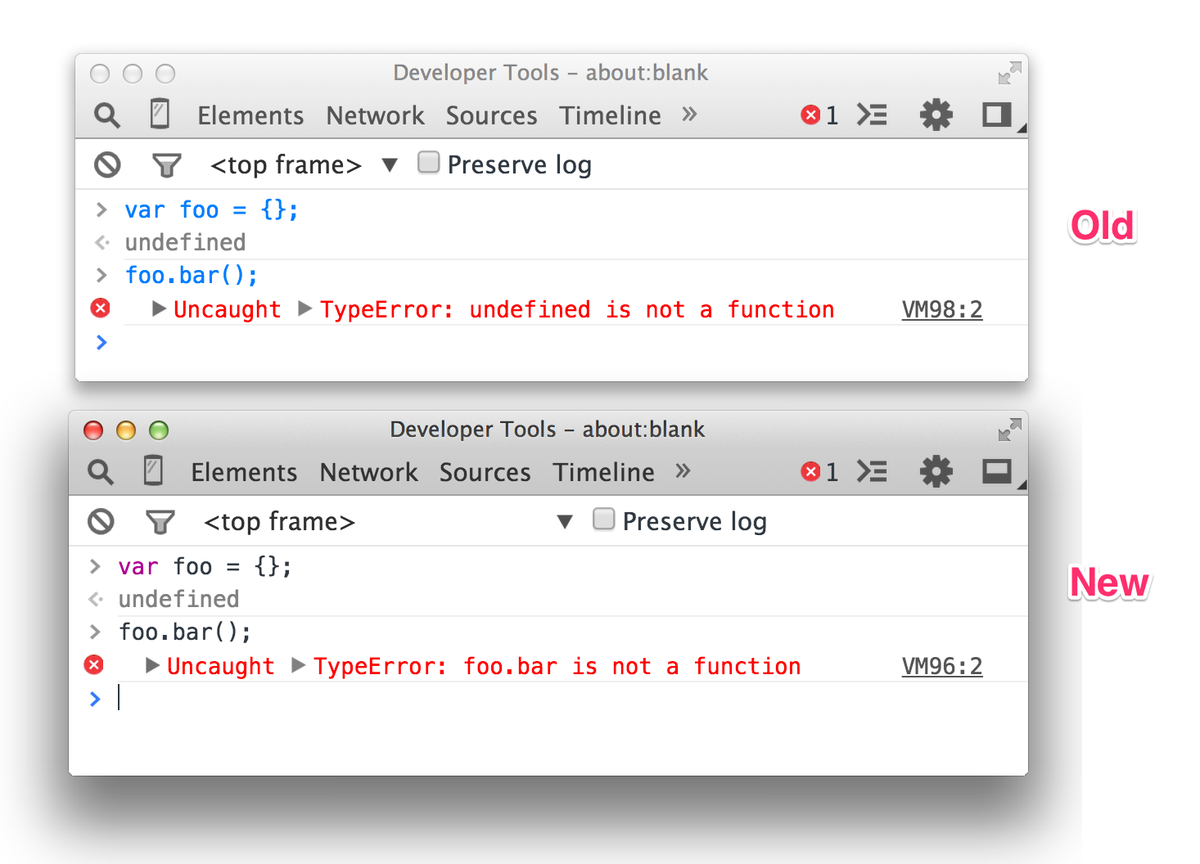
\includegraphics[width=1.0\linewidth]{assets/img/undefined-improved.png}
	\caption{Tweet by Addy Osmani (21-Feb-2015) announcing error report improvements in Chrome.}%
	\label{fig:undefined-improved}
\end{figure}

For JavaScript developers previous to 2015,
the error ``undefined is not a function'' was \comment{famous for not being helpful}{n\'ecessite une r\'ef\'erence}.
This error would very often rise from a typo somewhere in the code.
Due to the dynamic nature of JavaScript, the error can be reported late in the call stack.
Indeed, even if an error in the code might create an \verb|undefined| value,
it is only later when called, that an uncaught error would trigger.
As shown in Figure~\ref{fig:undefined-improved}, browsers are more helpful now,
at the cost of loosing an iconic error for all JavaScript developers.
Yet not having a compile step prevents advanced static analysis of the code,
and at the same time lengthen the feedback loop to fix errors.


\subsection{JavaScript as a compilation target}%
\label{sub:javascript_as_a_compilation_target}

As we now know, JavaScript exists since 1995, and from 1997 onward,
has mostly been the only way to run code dynamically in the browser.
For this reason, many alternative languages started treating JavaScript
as a compilation target to run code in a browser.

\subsubsection{Multi-tier programming}%
\label{ssub:multitier}

Haxe was probably the first production ready language to target JavaScript, in 2006.
At this time, there was no JIT, and JavaScript performances were fairly limited.
Some people were nonetheless trying to make the Web a video and gaming platform.
Flash, a multimedia platform running the ActionScript language was the most popular solution at the time.
In 2005, \textsf{YouTube} was for example relying on a Flash player to distribute videos.
Haxe was created by Nicolas Cannasse~\cite{haxe-interview} with the clear purpose
of removing the overhead of composing heterogeneous components like a Flash client,
a Web server, and additional JavaScript for Web games design.

Many other languages later followed that path of using the same language
for server and client code, sometimes called ``isomorphic'' frameworks,
or multi-tier programming environments.
Google announced their Google Web Toolkit (GWT) in May 2006~\cite{gwt},
enabling Java developers to build client applications.
The Ocsigen framework by V. Balat et al.~\cite{balat2006ocsigen} in 2006
allowed building Web applications in the OCaml programming language.
The Opal compiler~\cite{opalrb} translates Ruby code into JavaScript,
enabling full stack Ruby Web applications.
Today, most programming languages can target JavaScript,
including Python, C, Erlang, Haskell, etc.

Around the same period, academic research has also been trying to solve
multi-tier web programming with unique new languages like Links
by E. Cooper et al.~\cite{cooper2006links},
or Hop by Serrano et al.~\cite{serrano2006hop} in 2006.
Those efforts are continuing with for example
A. Chlipala et al.~\cite{chlipala2015ur} who created the Ur/Web variant
of the Ur modeling language,
or Sinha et al.~\cite{sinha2015simplifying} with the WebNat programming language in 2015.
According to~\cite{sinha2015simplifying} however,
experienced Web developers require fine grained control of the generate code,
debugging tools, deployment and configurations features
for designing complex real-world Web applications.
Unfortunately, those research attempts at novel ways of programming the Web
are not mature enough yet to be adopted by developers.

\subsubsection{JavaScript as the main target}%
\label{ssub:javascript_as_the_main_target}

Instead of trying to tackle both server and client-side programming,
a new category of languages later emerged, focusing on the client side,
and with JavaScript being the only or main compilation target.
The most notable ones are CoffeeScript~\cite{coffeescript} released in 2009
by Jeremy Ashkenas, Dart~\cite{dart-blog} designed by Lars Bak
(creator of the V8 engine) and Kasper Lund for Google in 2010,
Elm~\cite{czaplicki2013asynchronous} the product of Evan Czaplicki senior thesis
on functional reactive programming in 2012,
and Reason~\cite{reason} (also known as ReasonML) in 2016 by Jordan Walke (who is
also the original designer of the React framework we will discuss later).

One can notice that appart from Dart, which is heavily object-oriented,
those new languages follow the functional paradigm.
It may be related to guaranties brought by functional programming
that we will develop when exploring the Elm programming language.

\comment{}{A: sur cette section je reste un peu sur ma faim ; tu listes des frameworks, tu dis qu'ils sont fonctionnels pour des raisons qu'on d\'etaillera plus tard mais cela apporte finalement assez peu d'info}
\comment{}{M: Ok, alors c'est pas des frameworks, c'est des languages de programmation.
Mais contrairement à la section précédente, ce ne sont pas des languages pré-existants
qui ont été adaptés pour générer du JS,
mais des language créés spécifiquement dans le but de faire du frontend web.
Et contrairement aux sections suivantes, ce ne sont pas juste des superset ou légère
variations de JS.
Peut-être je devrais mettre en avant le fait que si tant de nouveaux languages
sont créés from scratch spécifiquement dans le but de générer du JS,
c'est parce qu'il y a un vrai besoin de diversité et d'approches différentes de JS pour le Web ?}

\subsubsection{Gradually typed JavaScript}%
\label{ssub:gradually_typed_javascript}

Coding with a completely different language is a rather extreme approach
which can be disturbing for developers.
From this observation, both Microsoft and Facebook decided to bring
new contributions to the JavaScript ecosystem under the form of gradual typing.
Gradual typing is a type system where values are partially typed.
Some may be typed, and consequently static typing rules are verified,
and some may be untyped, left for compile-time verifications.

In October 2012, Microsoft released TypeScript~\cite{bierman2014understanding},
a superset of JavaScript, introducing optional type annotations.
As a consequence, any valid JavaScript program is also a valid TypeScript program.
This property was most certainly the major success factor of TypeScript.
Programs can be ported progressively to benefit from static analysis.
Listing~\ref{lst:add-ts} exhibits the core type annotation feature of TypeScript.

\lstinputlisting[%
	language=JavaScript,
	caption={JavaScript and TypeScript version of an add function.},
	label={lst:add-ts}
]{assets/code/add.ts}

Another benefit of static typing that JavaScript developers are discovering when
switching to TypeScript is the improved IDE support,
which includes for example better autocompletion tools, jumping to definitions, etc.

In 2014, another tool named Flow and led by Facebook~\cite{chaudhuri2017fast}
enabled gradual typing of JavaScript.
Ultimately, TypeScript seems to be the most popular one,
but choosing between the two will most likely depend on how well they integrate
with the JavaScript framework and tools used in the corresponding application.

\subsubsection{JavaScript transpilation}%
\label{ssub:javascript_transpilation}

Despite increasing language complexity
as explained in Section~\ref{ssub:organic_growth_and_backward_compatibility},
ES2015 and later specifications brought very appreciated new features,
often influenced by other languages like CoffeeScript.
The \verb|async / await| pair of keywords is such example of syntax
reducing complexity of the code control flow.
New specifications, however, are not always immediately available in all browsers,
especially mobile versions.
But there exists one version of JavaScript fully supported on all browsers, ES5.
Inspired by the \comment{traceur}{TO BE CHECKED} tool by Google engineers,
Sebastian McKenzie started writing \textsf{6to5}~\cite{babel}
on September 2014, at the age of 17.
His \textsf{6to5} project, now renamed \textsf{Babel}, is known as a JavaScript ``transpiler'',
i.e.\ a program converting recent JavaScript source code into another (older) version
of JavaScript source code.
Today, \textsf{Babel} has become one of the most popular tools
with 7 million weekly downloads on \textsf{npm}.


\section{Frontend Web programming}%
\label{sec:frontend_web_programming}


\subsection{Single Page Application (SPA)}%
\label{sub:single_page_application_spa_}

In a desire to improve user experience in Web applications,
code location has progressively been shifting from server to client.
Since 2009, a Web framework named AngularJS~\cite{hevery2009declarative} strongly pushed
the Web actors toward writing ``Single Page Applications'' (SPA).
A Single Page Application gets its name from the fact that only one
HTML page is sent to the client browser.
This page however, contains JavaScript code taking control
of the application and rendering it for the rest of the user navigation.
When new data is required, the application can send requests
with the XMLHttpRequest (XHR) object, or a WebSocket provided by the browser,
then process the answer and re-render the HTML page accordingly.
Since February 2005, this technique was popularized under the name Ajax~\cite{ajax}
by Jesse James Garret and is represented in Figure~\ref{fig:spa}.
Ajax stands for asynchronous JavaScript and XML,
though today data is mostly exchanged in the JSON format (JavaScript Object Notation) instead of XML,
and occasionally just raw bytes depending on use cases and protocols.

\begin{figure}[ht]
	\centering
	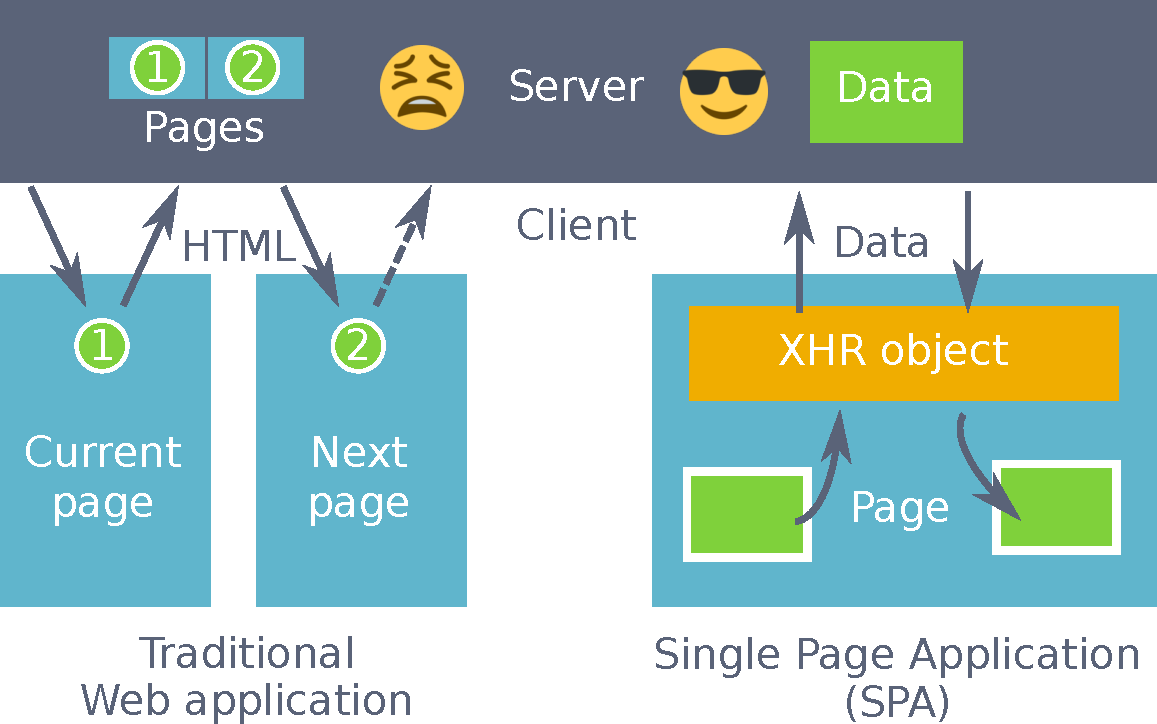
\includegraphics[width=1.0\linewidth]{assets/img/spa-bis.pdf}
	\caption{Difference between traditional Web applications and Single Page Application (SPA). A traditional application will ask the server to generate a new HTML page to access the required content. A SPA will just ask for the required data and render it in the client directly.}%
	\label{fig:spa}
\end{figure}


\subsection{Reactive programming}%
\label{sub:functional_reactive_programming}

In 2007, Sean Parent gave a talk at Google~\cite{parent2007talk, parent2007pdf}
on declarative user interface logic and building
the "Property Model Library" at Adobe~\cite{jarvi2008property}.
An analysis of Adobe's desktop applications code highlighted that a third of it
is devoted to event handling logic,
and that half of the bugs exist in this portion of the code.

Reactive programming is a paradigm focusing on manipulation of time-varying values.
It is especially suited for event-driven applications such as graphical user interfaces (GUI),
and tries to solve many of the issues brought by asynchronous callbacks.
Spreadsheet softwares for example, are usually implemented as reactive systems
in which modification of a cell will propagate to all computed cells depending on it.
In a survey on reactive programming~\cite{bainomugisha2013survey},
E. Bainomugisha et al. classify approaches along six axes:
representation of time-varying values, evaluation model, lifting operations,
multidirectionality, glitch avoidance, and support for distribution.

Representation of time-varying values and lifting operations
mostly depend on the underlying programming language.
Statically typed languages, will require a differentiation in the type
between a normal value and a time-varying one,
thus also needing "lifting" operations i.e. ways of transforming
functions working on regular values (like sum of two numbers)
into functions that operate on their time-varying version.
Dynamically type languages may figure this out at runtime,
and consequently avoid usage of lifting operators.

The evaluation model can be of two kinds,
push-based, pull-based, and sometimes a mix of the two.
The most common evaluation mechanism is push-based,
meaning once a time-varying value changes,
it pushes the change to other values depending on it.
A pull mechanism however usually relies of lazy evaluation languages such as Haskell.
The major issue of pulling is that the system may suddenly
require many depending past values and that will often result high memory consumption
and program pauses due to burst of computations.
Push-based evaluation has the advantage of lower memory usage
and quicker response, but may introduce temporary inconsistent states called glitches
if propagation of changes are pushed in a wrong order.

Most research on the topic have occurred in the context
of functional reactive programming (FRP), following Fran~\cite{elliott1997functional} in 1997.
Almost none of those research projects however are being
picked up for use in production.
Even Elm~\cite{czaplicki2013asynchronous} that got some traction in the Web industry,
decided to move away from FRP~\cite{elm017farewell} with its 0.17 release in 2016.
The reason for the move in Elm and low adoption of reactive programming in general
is probably due to the big learning curve for the concepts.
A recent JavaScript "compiler" project named Svelte~\cite{harrissvelte}
is trying to reintroduce reactive foundations with minimal alterations
to the JavaScript language.
It is too soon to predict if this approach will be successful,
even though it is getting traction.

One important aspect of reactive programming that has been picked up however,
is the declarative nature of binding graphical user interfaces to the
underlying data such that when the data changes, the interface is automatically updated.
This is often called one-way or two-way data binding depending on if
modifications of the user interface also immediately pushes changes to the associated data.


\subsection{Virtual DOM}%
\label{sub:virtual_dom}

The document object model (DOM) is the hierarchical structure of elements
composing an HTML page.
In order to understand what a virtual DOM is, and why it is useful,
we first need to understand how the browser renders the DOM.

\begin{figure}[ht]
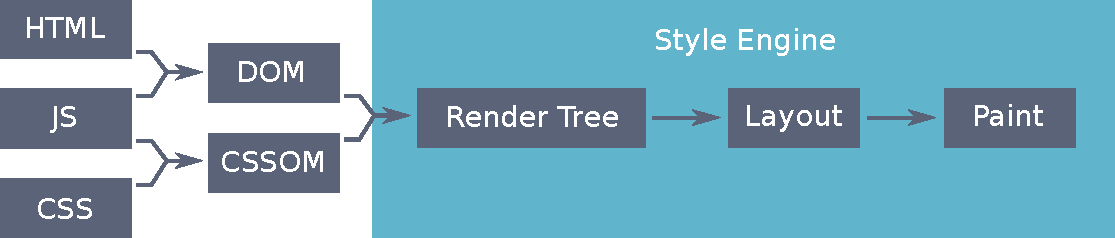
\includegraphics[width=\columnwidth]{assets/img/dom-rendering.pdf}
\caption{Rendering process of a Web page.}%
\label{fig:dom-rendering}
\end{figure}

The rendering process is depicted in Figure~\ref{fig:dom-rendering}.
First, the browser needs to build the DOM and the CSSOM trees.
The CSSOM is the equivalent of the DOM but for the hierarchy of CSS (styling) properties.
When combining the DOM and the CSSOM, the browser generates a render tree,
which contains all the visible nodes with their computed styles.
From the render tree, the browser can compute the layout of the page,
i.e. the exact position and sizes of all visible elements in the Web page.
Finally, the browser can ``paint'' the actual pixels on screen.
This used to be done in two phases,
first paint different virtual layers of related elements,
then compose and render those different layers on screen.
Recently, new rendering engines tend to combine those steps
into a process similar to those of game engines.
For more information on browsers rendering engine,
Lin Clark~\cite{clark-stylo, clark-webrender} also wrote
two enlightning blog posts on that subject.

In theory, everytime JavaScript code modifies the DOM or CSS properties,
the whole process should be called to rerender the page.
In practice, the browser framerate approximates the screen's one.
Therefore, the ``paint'' step only occurs roughly 60 times per second.
The layout however, may need to be recomputed at a higher framerate.
For example, reading the \verb|offsetX| and \verb|offsetY| properties
of a mouse event to get the current coordinates of the mouse while annotating images,
will require a reflow (recomputation of layout) if the DOM or CSSOM has changed.
Unfortunately that is exactly what we do when annotating images.
We retrieve mouse coordinates in the image,
and then draw the associated annotation on top.
This alternation of modifying the DOM and reading properties needing reflow
is the worst source of performance drops when happening at high frequencies.
Listing~\ref{lst:layout-reflow} is an example of code showcasing this issue.
Computing this loop with \verb|nbiter = 1000| takes 200ms on \textsf{Chrome}
while splitting the loop in two loops takes 3ms.

\lstinputlisting[%
  language=ES6,
  caption={Example code forcing layout recomputation by intertwining layout read and CSSOM write.},
  label={lst:layout-reflow}
]{assets/code/layout-reflow.js}

A virtual DOM is the combination of a data structure and an update mechanism
circumventing this kind of issues by batching all DOM modifications once per frame.
Instead of directly modifying the DOM,
one should modify the virtual DOM data structure.
Usually, the library providing the virtual DOM implementation will update the DOM at each frame
thanks to a diffing algorithm between the versions of the virtual DOM data structure at last frame
and at the new frame.
Representing the DOM as an intermediate data structure also have many benefits regarding testing
and enable writing pure visualization functions (not performing any side effect).

\subsection{How to choose?}%
\label{sub:how_to_choose_}

\subsubsection{Angular}%
\label{ssub:angular}

AngularJS~\cite{hevery2009declarative} dates back to 2009, when Miško Hevery and Adam Abrons
were trying to sell online storage services through software at getangular.com.
The project wasn't successful enough, and so they made <angular/> open source.
Miško Hevery was later recruited at Google to work on a new project.
The story, as told by Miško Hevery and Brad Green at Google I/O 2013~\cite{angularjs-googleio},
says that it took Miško three weeks (though he had bet two) to rewrite a six-month work
with 17000 lines of code into 1500 lines of code with <angular/>.
Impressed, Brad decided to embrace the <angular/> project under Google's wing
and it got rebranded AngularJS with a new logo.
In 2016, Google released its successor, renamed Angular (without the JS part).
An important difference is that Angular is using TypeScript instead of JavaScript.
The key feature of Angular/AngularJS is \comment{declarative two-way data binding,}
{Bien expliquer dans la partie reactive programming.}
showcased in Listing~\ref{lst:angularjs}.
Another important design decision is that Angular is trying
to provide a \comment{fully featured and coherant framework
capable of handling most use cases you will ever encounter.}
{trop vague, illustrer avec un example?}

\lstinputlisting[%
  language=HTML,
  caption={Two-way data binding in AngularJS.},
  label={lst:angularjs}
]{assets/code/angularjs.html}

\subsubsection{React}%
\label{ssub:react}

Contrary to Angular, React is designed to solve a very specific use case,
which is how to build user interfaces.
As such it doesn't care about how you store data,
or manage routing of the SPA with the url.
The core feature of React is its Virtual DOM \comment{that we will explain soon.}
{Bien expliquer dans la partie sur le VDOM}
It provides \comment{one-way data binding}{expliquer dans section reactive programming} between the state of a React component
and its rendering in the DOM.\@
The syntax used for the binding is showcased in Listing~\ref{lst:reactjs}.

\lstinputlisting[%
  language=ES6,
  caption={React example showing the state and render function of a component.},
  label={lst:reactjs}
]{assets/code/react.js}


\subsubsection{Vue}%
\label{ssub:vue}

\comment{Vue describes itself as a progressive framework,
meaning it provides core features targetting a small scope,
and other opt-in layers bringing more functionalities.
In a sense, it shares advantages and inconvenients of both
React and Angular, with a different balance point.
It mostly uses one-way data bindings,
but also provides inbuilt conveniences to simulate two-way data binding
through attaching event listeners when using the \texttt{v-model} property.}{Pas clair}
An example is given in Listing~\ref{lst:vuejs}.

\lstinputlisting[%
  language=HTML,
  caption={Simulated two-way data binding in Vue using the \texttt{v-model} property.},
  label={lst:vuejs}
]{assets/code/vue.html}


\subsubsection{Summary}%
\label{ssub:summary}

All three frameworks provide data binding between the state of the application
and its rendering, making the user interface declarative and reactive.
Angular and React are the more mature projects with
the biggest community.
Angular provides a solution covering most aspects needed for a SPA,
while React is focused on the user interface and will often be paired
with libraries to manage state efficiently like Redux.
\comment{Vue has a lower barrier to entry}{?}, like React,
but also a coherent set of opt-in functionalities making it an all-in-one solution similar to Angular.
In order to produce small application code compatible with most browsers,
one also should add transpilation, minification, and other preprocessing
tasks readying the code and assets for serving them on the Web.
We effectively end up making Web development similar
to static and compiled development environments.
Knowing all this, I will argue that we should instead use Elm,
a functional programming language compiling to JavaScript.
In the next section I will detail how it can bring
all the advantages of other Web frameworks,
but with an improved developer experience,
and a more reliable application at the end.

\section{Elm}%
\label{sec:elm}

\begin{displayquote}
	\textit{``Il semble que la perfection soit atteinte non quand il n’y a plus rien à ajouter,
	mais quand il n’y a plus rien à retrancher''}
	--- Antoine de Saint-Exupéry, Terre des Hommes, chapitre III, L'avion, 1939.
\end{displayquote}

Elm is a statically typed functional programming language for building Web applications.
Its syntax comes from the Meta Language (ML) family of languages, similar to Haskell and OCaml.
It strives for simplicity by removing non essential features
like custom operators in version 0.19,
and by avoiding functional programming jargon such as monads, functors, etc.
The home page of the language claims that Elm generates JavaScript
with great performances and no runtime exceptions.
In the following sections, we will see how its properties enable such a claim.

\subsection{Pure functions}%
\label{sub:pure_functions}

All functions in Elm, except for debugging, are ``pure'',
meaning they produce no side effect.
A side effect is a behavior with implications outside of the scope of a function,
such as modifying a global variable or an input parameter,
generating random values or interacting with the outside world.
Side effects are important to handle to build applications that are not predetermined
at startup, but we will explain later how they are managed withing The Elm Architecture (TEA).

Listing~\ref{lst:sideeffectjs} gives examples of functions that cannot be directly
translated from JavaScript to Elm due to side effects.
Pure functions are also sometimes called ``referentially transparent''
though the meaning of this terminology is unclear depending on sources.
The important property is that calling a pure function with the same arguments
will always return the same result.
As a consequence many optimizations can be performed such as memoization,
or precomputation of functions with no arguments (which actually are constant expressions).
The Elm compiler doesn't precompute constant expressions yet,
but memoization in the form of lazy functions can be used for computation
of view functions, reducing the amount of work for the diffing algorithm
of the virtual DOM.\@

\lstinputlisting[%
  language=ES6,
  caption={Side effects in JavaScript.},
  label={lst:sideeffectjs}
]{assets/code/side-effect.js}


\subsection{Algebraic Data Types (ADT)}%
\label{sub:algebraic_data_types_adt_}

Algebraic data types (ADT) initially appeared in 1980 with the Hope programming language,
developed by Rod Burstall, Dave MacQueen and Don Sannella~\cite{burstall1980hope}.
Since then, they have been popularized by functional programming languages
such as Haskell or OCaml.
Usually, algebraic data types include product types and sum types.
Product types are types regrouping multiple data together under the same name.
Tuples like (Int, Float), and records (or objects) are the most common product types.
Their names come from the properties on cardinality if we consider types as sets.
Indeed, a tuple of three booleans have a cardinality of 8 if you consider
all possible combinations, which is the product $2\times2\times2$.
Sum types are referred to as ``custom types'' in Elm terminology.
They are defined with the \verb|type| keyword.
Few examples of custom types definitions are provided in Listing~\ref{lst:customtype-elm}.
\comment{}{OneOfThreeBools as 6 distinct elements, 2 + 2 + 2}

\lstinputlisting[%
  language=Elm,
  caption={Custom types definitions in Elm.},
  label={lst:customtype-elm}
]{assets/code/customtype.elm}

The most important property of custom types in Elm
is that they enable modelization of a problem with exactly the correct
cardinality for the types, preventing impossible states by design.
Concretely, consider that we are modeling accessibility of a site
depending on the logged status of users.
Typically, in a language without sum types, like JavaScript,
the user will be modeled with two fields as in Listing~\ref{lst:userjs}.
Initially the \verb|loggedIn| field will be false and the user name empty.
As soon as the user is logged in,
the corresponding field will have the value \verb|true|,
and the name will be filled with the user name.
But what happens when the \verb|loggedIn| field is \verb|false| and
the name is filled with something like ``John Doe''.
In theory this state should never be reached if we are carefull in our implementation,
but in practice, bugs tend to fill every possible crack,
requiring more tests to verify that this state is never reached.
With custom types in Elm, the user type will be defined as in Listing~\ref{lst:userelm}.
In this definition, a user can either be anonymous or logged in with a name,
but never anonymous and with a name.
By design, custom types prevents an entire family of bugs.

\lstinputlisting[%
  language=ES6,
  caption={User modeled with a product type in JavaScript.},
  label={lst:userjs}
]{assets/code/user.js}

\lstinputlisting[%
  language=Elm,
  caption={User modeled with a custom (sum) type in Elm.},
  label={lst:userelm}
]{assets/code/user.elm}


\subsection{Total functions}%
\label{sub:total_functions}

Functions are qualified as ``total'' when they are guarantied
to return a result for every possible valid input.
\comment{}{Actually find a precise definition here.}
\comment{}{Advantages of total functions.}
Elm has two properties helping in the quest of total functions,
\begin{itemize}
	\item exhaustive pattern matching on custom types,
	\item and no statement, only expressions.
\end{itemize}

\subsubsection{No statement, only expressions}%
\label{ssub:no_statement_only_expressions}

In most programming languages like JavaScript,
programs are composed of successions of statements and expressions.
The former do not return values while the latter do.
Appart from imports, Elm code contains only top level definitions and expressions.
Listing~\ref{lst:expressionelm} provides example of Elm expressions
for conditions or loops.
All branches of conditions (\verb|if| expressions) must have a value of the same type.
Without an \verb|else|  branch, the code will not compile.
Not having \verb|for| loops statements is among the toughest functional
concepts to learn for beginners.
In a language with only expressions,
loops need to be expressed either with recursive functions,
or with higher order functions, like \verb|List.foldl| in the length example.

\lstinputlisting[%
  language=Elm,
  caption={Branching control and loops are expressions in Elm.},
  label={lst:expressionelm}
]{assets/code/expression.elm}


\subsubsection{Pattern matching}%
\label{ssub:pattern_matching}

Pattern matching is a branching mechanism based on the structure of a type.
Any custom type can be matched to one of its different variants
with the \verb|case ... of| syntax as shown in Listing~\ref{lst:pattern-matching-elm}.
Any lowercase variable in the pattern will be bound to the corresponding data,
like the \verb|name| variable here.

\lstinputlisting[%
  language=Elm,
  caption={Pattern matching in Elm},
  label={lst:pattern-matching-elm}
]{assets/code/pattern-match.elm}

In javascript, one can fairly easily forget to handle a case,
or willingly only process the ``happy path'' for prototyping speed.
In Elm, if I remove the \verb|Anonymous| branch,
the compiler will refuse to compile the code
with the message showed in Listing~\ref{lst:missing-pattern-elm}.
This is the main reason why the \verb|Nothing| value in Elm,
approximately equivalent to the \verb|null| value in JavaScript
will never trigger a runtime exception.
Everywhere it may appear, i.e.\ everywhere the \verb|Maybe| type is used,
Elm will guaranty at compile type that this case is handled.

\lstinputlisting[%
  language=Elm,
  caption={Missing pattern compiler error in Elm},
  label={lst:missing-pattern-elm}
]{assets/code/pattern-match-missing.elm}

As suggested in the hint of the compiler error,
we could also use \verb|Debug.todo "message"| in the \verb|Anonymous| branch,
which is very useful for the rapid prototyping phase.
Remark that the \verb|Debug.todo| function will make the program crash
if reached at runtime.
For this reason, all functions from the \verb|Debug| module
are forbidden in code compiled in release mode.


\subsubsection{No runtime exception}%
\label{ssub:no_runtime_exception}

Thanks to expressions and exhaustive pattern matching,
Refactoring an Elm code base can be done with confidence.
Any place where types do not match with functions
will be signalled by the compiler, which becomes a true coding assistant.
Noredink, a company based in San Francisco reported in 2018 that after
two years of using Elm in production,
they got their first runtime exception,
compared to 60000 for the JavaScript code~\cite{zeroruntimeerror}.


\subsection{The Elm Architecture (TEA)}%
\label{sub:the_elm_architecture_tea_}

\begin{figure}[ht]
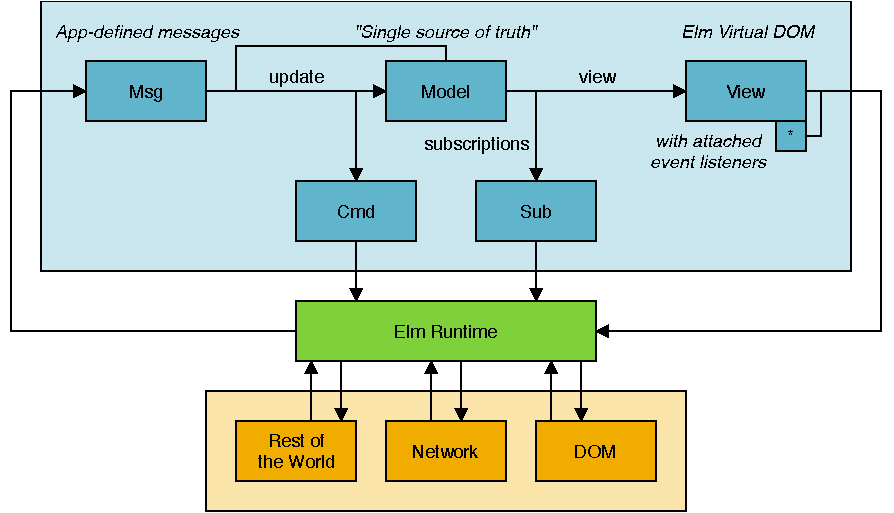
\includegraphics[width=\columnwidth]{assets/img/tea-draw-io.pdf}
\caption{The Elm Architecture (TEA).}%
\label{fig:tea}
\end{figure}

The Elm Architecture (TEA) enforces a unidirectional data transformation flow,
visualized in Figure~\ref{fig:tea}.
The central entity is the \verb|Model|.
It contains all and every information about our application state.
The visual aspect of our application is called the \verb|View|
(basically an HTML rendered document) which is generated by the \verb|view| function,
from the \verb|Model|. Finally, all events generate messages, of type \verb|Msg|.
The \verb|update| function, updates the model by reacting to those messages, closing the loop.

All functions are pure, meaning there is no side effect,
outputs of functions are entirely defined by inputs.
There cannot be global variables mutations,
real world events, network interaction etc.
Basically such a program would be running in a predestined way
from its start to its end,
preventing us from loading images and interacting with them.
This is why the application is attached to the Elm runtime,
provided by the language, transforming all real world events (``side effects'')
into our defined set of messages, of type \verb|Msg|.

The main challenge with pure functions is
to describe side effects without performing them.
Those are described in three locations:

\begin{enumerate}
\item View attributes as DOM event listeners for pointer events.
\item Commands (\verb|Cmd|) generated by the update function, like loading of images.
\item Subscriptions (\verb|Sub|) to outside world events like the window resizing.
\end{enumerate}

The Elm runtime takes those side effect descriptions,
perform them, and, whenever there is a result / an answer,
transforms it into one of our defined messages (\verb|Msg|)
and routes it to our update function.
After updating the model, the runtime automatically calls the \verb|view| function.
This way, the user interface reacts to model modifications
similarly than with other one-way data bindings we have previously introduced.


\subsection{Elm-UI, an alternative layout strategy}%
\label{sub:elm_ui_an_alternative_layout_strategy}

\begin{figure}[ht]
	\centering
	\setlength{\fboxsep}{0pt}
	\fbox{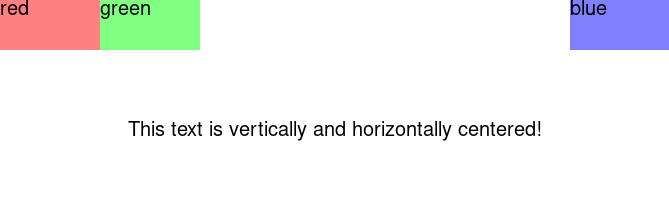
\includegraphics[width=1.0\linewidth]{assets/img/elm-ui.png}}
	\caption{User interface specified by Listing~\ref{lst:elm-ui}.}%
	\label{fig:elm-ui}
\end{figure}

We have seen that the Elm architecture enables building Web applications with HTML views.
It treats the user interface as data, using a virtual DOM under the hood
and managing the DOM side effects with a runtime system.
Overall, with Elm guaranties, one is fairly confident that when
the program compiles, it is functionally correct.
Layout however, traditionally relies both on HTML and CSS rules,
intrinsically hard to debug due to their cascading nature
since a CSS rule may apply to all children of a DOM element.
In~\cite{sinha2015simplifying}, Sinha et al. identified user interface design
as the main difficulty in Web development.

At Elm Europe 2017, Matthew Griffith made a presentation
entitled ``Understanding style''~\cite{griffithstyle}.
In this work, he identifies the most problematic aspect of layout being
that there is no clear way to identify when it is incorrect.
There is not even an unhelpful ``undefined is not a function'' error in CSS resolution.
Basically an error in layout and style is just the unexpected.
With this in mind he created library, now named elm-ui~\cite{griffithelmui},
aiming at providing the guaranty that if your code compiles,
the layout if fully specified.
They key property of the library is that its base building block,
the \verb|el| element only has one child,
instead of a list like in the case of a \verb|div| HTML element.
Also, building blocks with multiple children must have explicit layout.
Listing~\ref{lst:elm-ui} showcases how functional composition of UI elements
and an attention on naming enable building of clear and robust user interfaces.
The corresponding user interface is provided in Figure~\ref{fig:elm-ui}.

\lstinputlisting[%
  language=Elm,
  caption={Fully specified layout with elm-ui.},
  label={lst:elm-ui},
  basicstyle=\scriptsize\ttfamily
]{assets/code/elm-ui.elm}


\subsection{Reliable packages}%
\label{sub:reliable_packages}


Elm packages are versioned using
the semantic versioning specification~\cite{semanticversioning},
with the MAJOR.MINOR.PATCH schema.
The major number is incremented when changes breaking the API are introduced,
such as removing a function or modifying its type signature.
The minor number is incremented when new values or functions are introduced.
Finally the patch number is incremented when nothing else than internal
non-exposed implementation are modified.
Since Elm uses total functions, it is able to programmatically compute
version number increments with the \verb|elm bump| command.
As a consequence, upgrading your dependencies is guarantied by the compiler
to not break one code as long as they don't increase the major number.

Another advantage of having pure, total functions is that type signatures are not lying,
implying that one can immediately identify functions capable of triggering side effects.
At the current state of the Elm language,
the only places where side effects can happen are
ports to JavaScript (forbidden in packages), commands and HTML.
Therefore, a dependency that doesn't expose functions with commands or HTML
in their type signatures will not be able to steal bitcoins or launch nuclear warheads.
